%%% The main file. It contains definitions of basic parameters and includes all other parts.


%% Settings for two-sided (duplex) printing
\documentclass[10pt,a4paper]{report}
\let\openright=\cleardoublepage

%% Character encoding: usually latin2, cp1250 or utf8:
\usepackage[utf8]{inputenc}

%% It's 2019
\usepackage[default]{droidserif}
\usepackage[T1]{fontenc}

%% Further useful packages (included in most LaTeX distributions)
\usepackage{amsmath}        % extensions for typesetting of math
\usepackage{amsfonts}       % math fonts
\usepackage{graphicx}       % embedding of pictures
\usepackage{tikz}
%\usetikzlibrary{shapes,fit,positioning,snakes,mindmap,trees,decorations.text,arrows.meta}
%\makenomenclature
\usepackage{algorithm,algpseudocode}
\usepackage{booktabs}
\usepackage{mwe}
\usepackage{afterpage}
\usepackage{pgfgantt}
\usepackage{pdflscape}
\usepackage{geometry}
\usepackage{enumitem}
\usepackage{float}
\usepackage{framed}
\usepackage{titlesec}
\usepackage{listings}
\usepackage{xcolor}
\usepackage{longtable}
\usepackage{makecell}
\usepackage[toc,page]{appendix}
\usepackage{multirow}
\usepackage{tocbibind}
\usepackage{etoolbox}
\usepackage{fancyvrb}
\usepackage[font=small,labelfont=bf]{caption}
\usepackage{listings}
\usepackage[obeyspaces]{url}

\lstset{basicstyle=\ttfamily,
	showstringspaces=false,
	commentstyle=\color{red},
	keywordstyle=\color{blue}
}

\usepackage{pdfpages}

\usepackage[textsize=tiny,backgroundcolor=yellow!50, linecolor=black!25]{todonotes}

% links shall be clickable
\usepackage[unicode]{hyperref}   % Must follow all other packages
%\usepackage{cleveref} % Must follow all other packages including hyperref
\usepackage[noabbrev]{cleveref}
\AtBeginEnvironment{appendices}{\crefalias{chapter}{appendix}}

% indexing
\usepackage{makeidx}
\makeindex
\usepackage[totoc, columns=1]{idxlayout}
% Definitions of macros (see description inside)

\newcommand{\cool}{\color{green!50!white!80!black}}
\newcommand{\textcool}[1]{{\cool #1}}

\newcommand{\XX}[1]{\textcolor{red}{#1}}
\newcommand{\TT}[1]{\texttt{#1}}
\newcommand{\SC}[1]{{\fontfamily{phv}\selectfont\textsc{#1}}}

% Draw black "slugs" whenever a line overflows, so that we can spot it easily.


% avoid some slugs naturally
\clubpenalty=1000
\widowpenalty=1000
%\hyphenpenalty=100  % turn this on to prevent hyphenation
\emergencystretch=2cm


%%% The field of all real and natural numbers
\newcommand{\R}{\mathbb{R}}
\newcommand{\N}{\mathbb{N}}
\newcommand{\F}{\mathbb{F}}
\newcommand{\Z}{\mathbb{Z}}

\newcommand{\bms}{\begin{enumerate}[label=\bf (M\arabic*)]}
\newcommand{\bwp}{\begin{enumerate}[label=\bf \normalsize  (WP\arabic*), resume=del]}
\newcommand{\eenum}{\end{enumerate}}
\newcommand{\itemm}{\large \item }
\newcommand{\itemwp}{ \normalsize \item }
\newcommand{\deadline}[2]{\small (deadline: \textit{month #1}, duration: \textit{#2 moths})}
\newcommand{\people}[1]{\textit{\small (#1)}}


% move the headings out of gutenberg era
\setcounter{secnumdepth}{4}
\titleformat{\chapter}{\cool\fontsize{24pt}{24pt}\bfseries}{\color{black!25}\thechapter.}{1em}{}
\titleformat{\section}{\cool\fontsize{16pt}{18pt}\bfseries}{\scriptsize\color{black!25}\thesection}{1em}{}
\titleformat{\subsection}{\cool\fontsize{12pt}{14pt}\bfseries}{\scriptsize\color{black!25}\thesubsection}{1em}{}
\titleformat{\subsubsection}{\cool\bfseries}{\scriptsize\color{black!25}\thesubsubsection}{1em}{}

% code floats
\colorlet{shadecolor}{cyan!10}
\makeatletter
\newcommand\floatc@code[2]{{\@fs@cfont #1} #2\par}
\newcommand\fs@code{\def\@fs@cfont{\bfseries}\let\@fs@capt\floatc@code
\def\@fs@pre{}%
\def\@fs@mid{\vspace{-.5ex}\begin{shaded}}%
\def\@fs@post{\vspace{-1em}\end{shaded}}%
\let\@fs@iftopcapt\iftrue}
\makeatother

\floatstyle{code}
\newfloat{listing}{tbp}{lst}
\floatname{listing}{Listing}

% file indexing
\makeatletter
\def\patheach#1#2#3{\@test@patheachF{#1}{#2}#3/\endgroup}
\def\@test@patheachF#1#2#3\endgroup{\if#3\empty\empty\else\@patheachF{#1}{#2}#3\endgroup\fi}
\def\@patheachF#1#2#3/{#1{#3}\@test@patheach{#1}{#2}}
\def\@test@patheach#1#2#3\endgroup{\if#3\empty\empty\else\@patheach{#1}{#2}#3\endgroup\fi}
\def\@patheach#1#2#3/{#2#1{#3}\@test@patheach{#1}{#2}}
\def\foreach#1#2{\@test@foreach{#1}#2,\endgroup}
\def\@test@foreach#1#2\endgroup{\if#2\empty\empty\else\@foreach{#1}#2\endgroup\fi}
\def\@foreach#1#2,{#1{#2}\@test@foreach{#1}}
\makeatother

\def\makefileindex#1{%
\index{\patheach{\texttt}{!}{#1}}%
\hspace{-1ex}\texttt{\patheach{}{/\-}{#1}}\\}

\def\makefileindexnotext#1{%
	\index{\patheach{\texttt}{!}{#1}}}

\def\makefileindexes#1{\foreach{\makefileindex}{#1}}

\newcommand{\srcstyle}[1]{\tt\scriptsize\textcolor{gray}{\makefileindexes{#1}}}
\newcommand{\sectionFiles}[2]{ \strut~\hfill~\hspace{1ex}~\parbox{#1}{\tt\scriptsize\textcolor{gray}{\makefileindexes{#2}}}}

\newcommand{\chapterSrc}[3][.4\linewidth]{\chapter[#2]{#2\sectionFiles{#1}{#3}}}
\newcommand{\sectionSrc}[3][.4\linewidth]{\section[#2]{#2\sectionFiles{#1}{#3}}}
\newcommand{\subsectionSrc}[3][.4\linewidth]{\subsection[#2]{#2\sectionFiles{#1}{#3}}}
\newcommand{\subsubsectionSrc}[3][.4\linewidth]{\subsubsection[#2]{#2\sectionFiles{#1}{#3}}}

% index typesetting customization
\renewcommand\indexname{Source file documentation index}
\providecommand*\lettergroup[1]{}
\makeatletter
\newcommand\idxitem{\@idxitem}
\newcommand\idxIitem{\@idxitem\texttt{.\ }}
\newcommand\idxIIitem{\@idxitem\texttt{.\ .\ }}
\newcommand\idxIIIitem{\@idxitem\texttt{.\ .\ .\ }}
\newcommand\idxIIIIitem{\@idxitem\texttt{.\ .\ .\ .\ }}
\newcommand\idxIIIIIitem{\@idxitem\texttt{.\ .\ .\ .\ .\ }}
\makeatother

% Include large PDFs
\newenvironment{foldoutfloat}{%
	\eject\pdfpageheight=52cm\pdfpagewidth=40cm
	\newgeometry{margin=1in}
	\textwidth=15in
	\begin{figure}[p]
	}{%
	\end{figure}
	\clearpage % otherwise it will float to another, non-resized page
	\eject\pdfpageheight=11in\pdfpagewidth=8.5in
	\restoregeometry
}

\newenvironment{foldoutfloatlandscape}{%
	\eject\pdfpageheight=40cm\pdfpagewidth=52cm
	\newgeometry{margin=1in}
	\textwidth=15in
	\begin{figure}[p]
	}{%
	\end{figure}
	\clearpage % otherwise it will float to another, non-resized page
	\eject\pdfpageheight=11in\pdfpagewidth=8.5in
	\restoregeometry
}%


\title{\textcool{\bf SOMHunter Video Search Tool} \\ Developer Documentation}
\author{František Mejzlík, Vít Škrhák, Patrik Veselý}
\date{Supervisor: doc. RNDr. Jakub Lokoč, Ph.D. \\ \vspace{5mm} Consultant: Mgr. Ladislav Peška, Ph.D.}

% Title page and various mandatory informational pages
\begin{document}
\maketitle

%%% A page with automatically generated table of contents of the bachelor thesis
\tableofcontents

%%% Each chapter is kept in a separate file



\chapter*{Acknowledgements}
Hereby, we'd like to thank our supervisor Jakub Lokoč as well as our consultant Ladislav Peška for their invaluable input to this project. For their great ideas, time and constructive feedback.

We thank Miroslav Kratochvíl for co-developing the first version of the tool with us. Also, for providing his EmbedSOM\footnote{https://github.com/exaexa/EmbedSOM} implementation and for the technical advice he's been giving us throughout the whole project.

Moreover, we thank Tomáš Souček that he allowed us to use and modify his extraction pipeline. Also for his help with the ranking server implementation.

\chapter{Prerequisites}
\section{Known-Item Search (KIS)}
The known-item search problem is defined as follows; a user is looking for a specific scene in a large video dataset. As an example, imagine yourself looking for a video you saw on some video streaming platform, but you don't remember the name. Or some of your friends are describing to you some specific funny moment they remember. That's the moment where the SOMHunter tool comes in to help. 

\section{Ad-hoc video search (AVS)}
The AVS problem, its definition says that a user is looking for all scenes matching his description. Therefore there is more than one correct answer to such a task. Imagine, you're looking for all the scenes where a dog rides a bike for example.

\chapter{Introduction}

SOMHunter is a prototype of an interactive video search tool designed specifically for known-item search (KIS) problems and is also well usable for Ad-hoc video search (AVS). Also in the past two years, SOMHunter competed in two Video Browser Showdown (VBS) sessions (2020, 2021), where we scored first and second places, respectively, in KIS tasks. On top of that, we took part in two Lifelog Search Challenges (LSC) (2020, 2021) where we managed to place ourselves as the second-best tool both of the times.

The tool features some powerful tools for the end-user to employ, but in a way that even novice users can grasp them in little time. Such concepts are natural language text search or similar frame "liking". Both of these concepts are well-known for the vast majority of users. Moreover,  SOMHunter offers other advanced features as well. Those are primarily meant for expert users, but at the same time don't stand in a way of novice users in any way.

SOMHunter is implemented as a modular cross-platform application with its user interface as a web application. Thanks to the web-based UI, the tool can also run in a setup where all parts run on a performant remote server and the end-user just uses it as a web app on a given URL. This is actually how we used SOMHunter in the last VBS and LSC competitions. Or you can run all the parts on your machine or an arbitrary combination of local and remote running parts.

\begin{figure}[b]
	\centering
	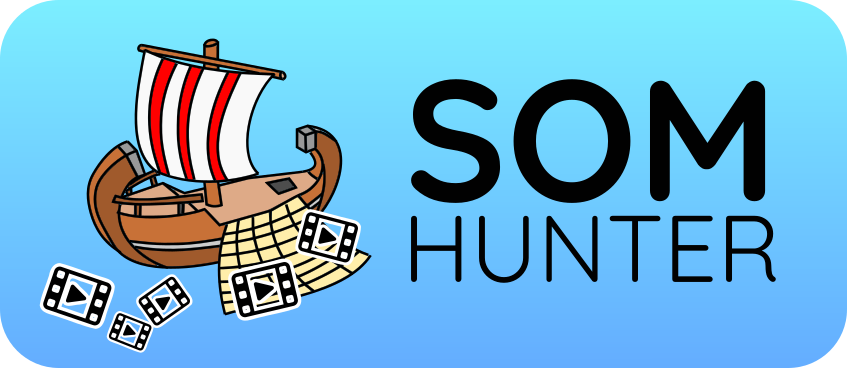
\includegraphics[width=0.7\textwidth]{img/somhunter-logo.png}
  \caption{\textbf{SOMHunter logo.}}
	\label{fig:logo}
\end{figure}


\part{Project overview}
\chapter{SOMHunter Overview}
\label{overview}


\begin{figure}
	\centering
	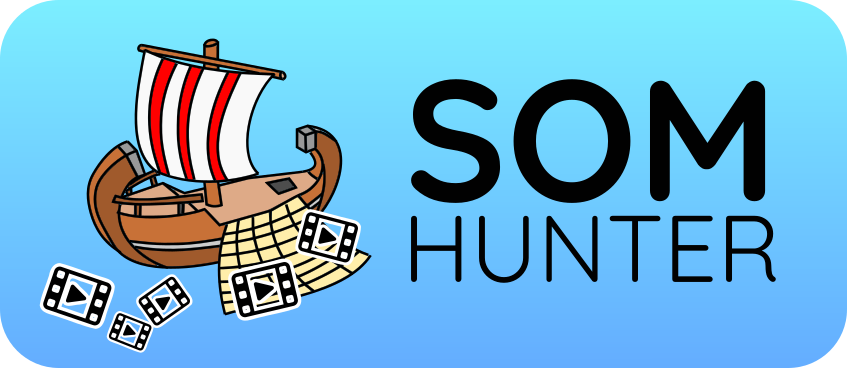
\includegraphics[width=\textwidth]{img/somhunter-logo.png}
	\label{fig:logo}
\end{figure}

\chapter{SOMHunter Architecture}
\label{arch}

\cref{fig:sh_arch}



\begin{figure}[b]
	\centering
	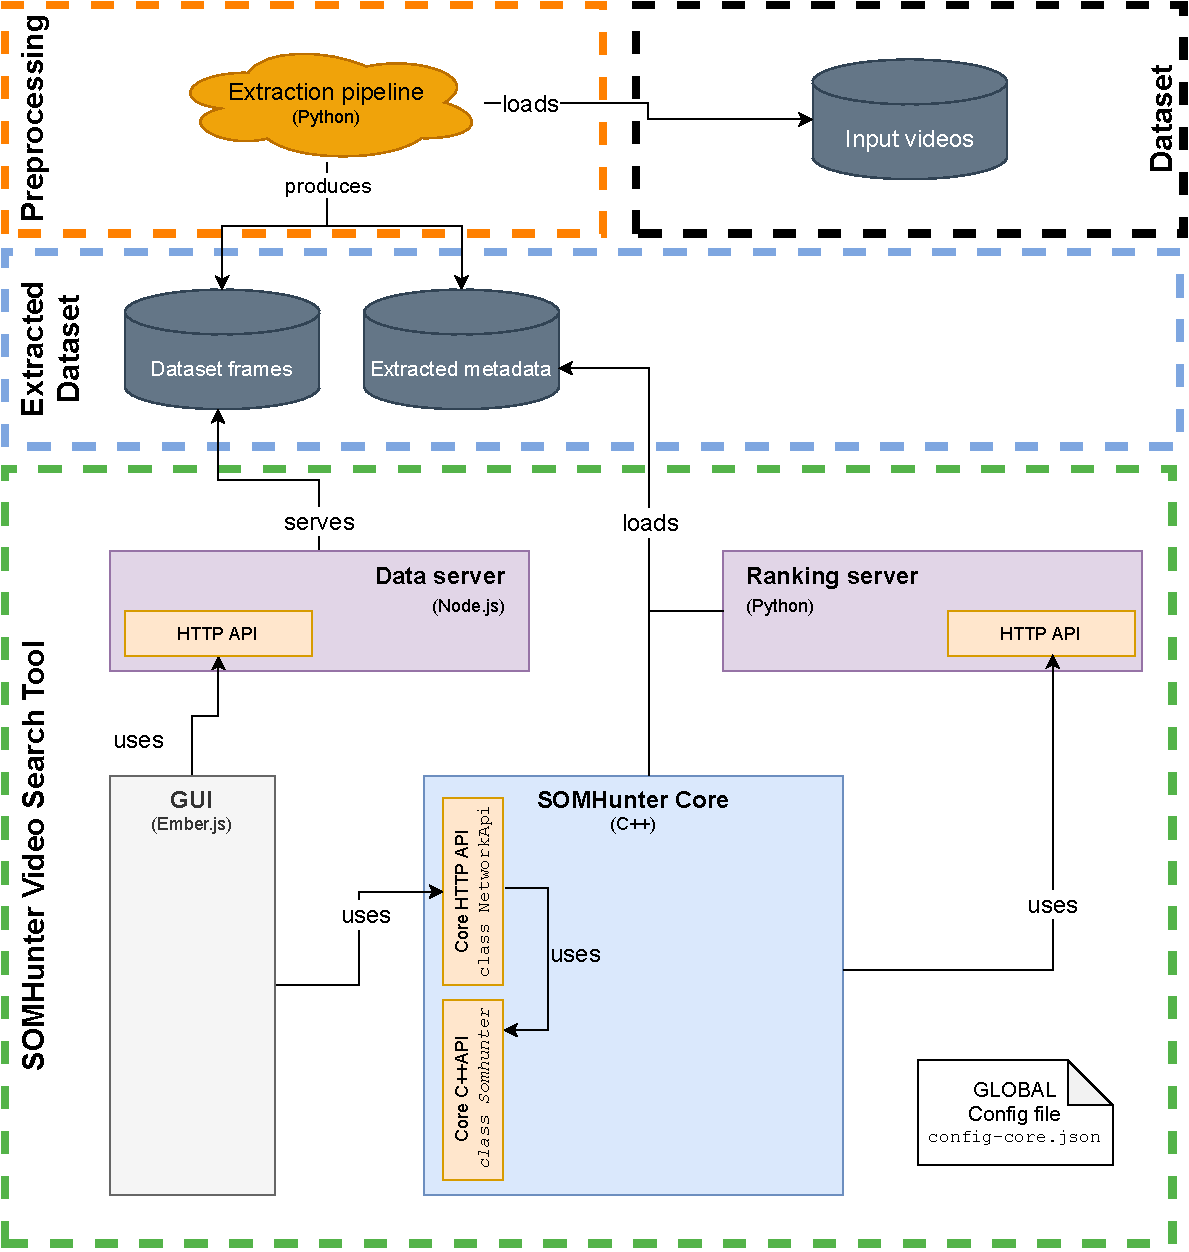
\includegraphics[width=1.0\textwidth]{img/diagrams/sh-arch.pdf}
	\caption{\textbf{High-level architecture of the SOMHunter tool.} Showing also extraction pipeline and visualising the path of the input dataset.}
	\label{fig:sh_arch}
\end{figure}


\part{System Components}
\chapter{Core}
\label{comp-core}

In this chapter we'll take a closer look at the core component and it's important parts.

\section{SOMHunter HTTP API}
That it just "translates" HTTP requests to C++ calls and vise versa with returned values.

\subsection{Endpoints \& OpenAPI}
What endpoints are supported? We are OpenAPI complaint.

\subsection{Implementation}
Describe why cpprestsdk...

https://github.com/microsoft/cpprestsdk

\subsection{Discussion on Implementation}

\paragraph{Pros}
\begin{itemize}
	\item + It is cross platform.
\end{itemize}

\paragraph{Cons}
\begin{itemize}
	\item - Has it's own JSON lib.
	\item + Not actively developed anymore.
\end{itemize}



\section{C++ API}

\section{Current Settings}

\section{Loaded Dataset}

\section{Rankers}

\section{Other Services}

\section{User Search Context (State)}


\chapter{UI}
\label{comp-ui}


\chapter{Data Server}
\label{comp-data-server}


\chapter{Ranking Server}
\label{comp-ranking-server}

The current ranking server is implemented in Python in the Flask framework. At the start, it loads the image features from the path specified in the \lstinline{CLIP_FEATURES} environment variable. 

Additionally, it requires a dimension of the features in variable \lstinline{CLIP_DIMENSION}. It supports two endpoints: \url{/clip/<query>} and \url{/clip-results/<query>}. The first endpoint takes the query part and embeds it into the CLIP\footnote{https://openai.com/blog/clip/} feature vector space. The second endpoint embeds the query the same way but on top of that, it computes distances to each image feature vector and returns an ordered list of results. It returns only a part of the result (restricted by count in environment variable \lstinline{HOW_MANY_RESULTS}).

\chapter{Extraction Pipeline}
\label{extraction-pipeline}


https://github.com/siret-junior/extraction-pipeline

\chapter{Extracted Dataset}
\label{extracted-dataset}


Describe the formats of the files.


\part{Other Supporting Software}
\chapter{SOMCollector}
\label{somcollector}

In this chapter, we will describe SOMCollector. This software was created for the user interaction logs collection and thus its possibilities are reduced in comparison to SOMHunter. In the following sections, I will describe the differences between SOMCollector and SOMHunter and what was added. This project has additional material in Czech like user manual and data description on wiki~\footnote{https://github.com/siret-junior/som-collector/wiki}. 

\section{HTTP and Core API}
In this version, the HTTP API is managed by the node.js layer and the core API is called through the node.js module system. The functionality of the core API is smaller than in SOMHunter because it was forked from a version that did not support that many features. The additions to the SOMHunter were three: multi-user support, a new specific type of logging, and a simplified search flow. The multi-user support is provided by \lstinline{class SomHuntersGuild} which holds SOMHunter objects for each user. The specific logging is implemented in \lstinline{FeedbackLogger} where it creates for each rescore call a single line CSV file. The logged format of the data is described in the wiki of the project~\footnote{https://github.com/siret-junior/som-collector/wiki -> Příručka k logovaným datům}. After the data collection, these files can be concatenated and the data analysis can be performed. The simplified version of the search flow was implemented mainly in the UI. In the core we added a target images sequence, that was read from a given file. The current target image was searched by a user and logged in the CSV file.

\section{UI}

The user interface is written in HTML and vanilla JS. The original SOMHunter UI from the older version was simplified only to enter a text query and show 64 frames. Additional features like gaining experience and levelling up were introduced to motivate users to search for a longer time. This was implemented mainly in the UI in function \lstinline{showSubmitWindow}.

\chapter{SOMHunter Simulator}
\label{somhunter-simulator}


https://github.com/siret-junior/somhunter-simulator

\chapter{Log Analyzer}
\label{log-analyzer}


https://github.com/siret-junior/log-analyzer


\part{Examples of Tool Extension}
\chapter{Example: Adding Custom Display}
\label{example-add-display}

\chapter{Example: Adding Custom Ranker}
\label{example-add-ranker}

\chapter{Example: Adding Custom Dataset}
\label{example-custom-dataset}


\part{Build Guide}
\chapter{Build instructions}
\label{build}

In this chapter, we will go through a build process of the main SOMHunter application. There will be presented two methods.

\section{Using Docker}

The easier build solution is via docker~\footnote{https://docs.docker.com/get-docker/} and docker-compose~\footnote{https://docs.docker.com/compose/install/}. Together with git~\footnote{https://git-scm.com/book/en/v2/Getting-Started-Installing-Git}, these are the only prerequisites for the build. Build steps:

\begin{enumerate}
  \item Clone SOMHunter repository
  \item \lstinline{sudo sh install-docker.sh RelWithDebubInfo}
  \item \lstinline{sudo docker-compose up}
\end{enumerate}

After everything is finished the UI of the application is running on address \url{http://localhost:8080}.

\section{Manual Build}

The manual build is harder because you have to get many prerequisites manually. This is the complete list of all prerequisites:

\begin{itemize}
  \item All the packages from \lstinline{build-essential}
  \item Git~\footnote{https://git-scm.com/book/en/v2/Getting-Started-Installing-Git}
  \item Python3~\footnote{https://www.python.org/downloads/} with alias python and urllib3 installed
  \item Node.js~\footnote{https://nodejs.org/en/} and npm~\footnote{https://www.npmjs.com/}
  \item Ember.js~\footnote{https://guides.emberjs.com/release/getting-started/quick-start/}
  \item libcurl~\footnote{https://curl.se/libcurl/}
  \item OpenCV~\footnote{https://opencv.org/}
  \item cpprestsdk~\footnote{https://github.com/microsoft/cpprestsdk}
\end{itemize}

Build steps:

\begin{enumerate}
  \item Clone SOMHunter repository
  \item Run main install script which calls recursively other install scripts \lstinline{sh install.sh RelWithDebugInfo}
  \item Start all the parts \lstinline{sh run.sh}
\end{enumerate}

Now we will describe the installation scripts in each project. The ranking server creates Python virtual environment and installs all the requirements in the \path{requirements.txt}. The data server and its dependencies from \path{package-lock.json} are installed and built by npm. Similarly, the UI's dependencies are installed and built by npm and then the UI is built by the ember extension. Finally, the core is built using CMake.


\part{Dependencies}
\chapter{Third-party Software}
\label{third-party}


\bibliography{biblio} 
\bibliographystyle{apalike}

\printindex
\begin{appendices}

\end{appendices}

\end{document}
